\documentclass[12pt]{article}
\usepackage{hyperref,amsmath,amsfonts,amssymb,fullpage,color,tikz}
\usetikzlibrary{decorations.pathmorphing,arrows.meta,patterns,calc}
\newcommand{\be}{\begin{equation}}
\newcommand{\ee}{\end{equation}}
\newcommand{\bh}{\bar{h}}
\usepackage{enumitem}
\newcounter{quesno}
\newcommand{\ques}[1]{\vspace{2em}\stepcounter{quesno}
\noindent{\bf Question \thequesno.} \emph{(#1 points)\\}
}

\begin{document}

\begin{center}
{\bf\Large General Relativity}

\vspace{1em}
{\bf\large Final Examination -- Model Solutions}
\end{center} 

\vspace{1em}
\hrule
\vspace{1em}

%==============================================================================
% QUESTION 1
%==============================================================================
\ques{2} 
\textbf{Problem Statement:} The components of the Riemann tensor in some coordinates are $R^\mu{}_{\nu\rho\sigma}$. Write down how they transform under a change of coordinates. Define the Ricci tensor by $R_{\mu\nu} = R^\rho{}_{\mu\rho\nu}$, and show explicitly that this transforms as a tensor under change of coordinates.

\medskip
\noindent\textbf{Solution:}

\noindent\textbf{1. Transformation of the Riemann tensor:}

Let $x^\mu \to x'^\mu(x)$ be a general smooth, invertible coordinate transformation. The components of the Riemann curvature tensor $R^\mu{}_{\nu\rho\sigma}$ are those of a $(1,3)$ tensor, meaning it has one contravariant (upper) index and three covariant (lower) indices. Under a change of coordinates $x^\mu \to x'^\mu$, its components transform according to the tensor transformation law:
\be
R'^\mu{}_{\nu\rho\sigma}(x') = \frac{\partial x'^\mu}{\partial x^\alpha} \frac{\partial x^\beta}{\partial x'^\nu} \frac{\partial x^\gamma}{\partial x'^\rho} \frac{\partial x^\delta}{\partial x'^\sigma} R^\alpha{}_{\beta\gamma\delta}(x) \,.
\ee

\medskip
\noindent\textbf{2. Transformation of the Ricci tensor:}

The Ricci tensor is defined in any coordinate system by contracting the first and third indices of the Riemann tensor:
\be
R_{\mu\nu} = R^\rho{}_{\mu\rho\nu} \,.
\ee
In the primed coordinate system $x'^\mu$, the components of the Ricci tensor are therefore defined by setting the third index equal to the first (and summing over the repeated index $\rho$):
\be
R'_{\mu\nu}(x') = R'^\rho{}_{\mu\rho\nu}(x') \,.
\ee
Substituting the transformation law of the Riemann tensor into this definition gives:
\be
R'_{\mu\nu}(x') = \frac{\partial x'^\rho}{\partial x^\alpha} \frac{\partial x^\beta}{\partial x'^\mu} \frac{\partial x^\gamma}{\partial x'^\rho} \frac{\partial x^\delta}{\partial x'^\nu} R^\alpha{}_{\beta\gamma\delta}(x) \,.
\ee
Using the chain rule for partial derivatives, the product of the Jacobian matrix and its inverse contracts to the Kronecker delta:
\be
\frac{\partial x'^\rho}{\partial x^\alpha} \frac{\partial x^\gamma}{\partial x'^\rho} = \frac{\partial x^\gamma}{\partial x^\alpha} = \delta^\gamma_\alpha \,.
\ee
Substituting this identity back into the expression for $R'_{\mu\nu}(x')$, we obtain:
\begin{align}
R'_{\mu\nu}(x') &= \delta^\gamma_\alpha \frac{\partial x^\beta}{\partial x'^\mu} \frac{\partial x^\delta}{\partial x'^\nu} R^\alpha{}_{\beta\gamma\delta}(x) \nonumber\\
&= \frac{\partial x^\beta}{\partial x'^\mu} \frac{\partial x^\delta}{\partial x'^\nu} R^\alpha{}_{\beta\alpha\delta}(x) \nonumber\\
&= \frac{\partial x^\beta}{\partial x'^\mu} \frac{\partial x^\delta}{\partial x'^\nu} R_{\beta\delta}(x) \,.
\end{align}
This is precisely the transformation law for the components of a rank $(0,2)$ covariant tensor under a general coordinate transformation. Hence, $R_{\mu\nu}$ transforms as a tensor.

\vspace{1em}
\hrule

%==============================================================================
% QUESTION 2
%==============================================================================
\ques{3}
\textbf{Problem Statement:} Consider a manifold on which we have both a metric, $g_{\mu\nu}$, and a totally antisymmetric $(0,3)$ tensor, $H_{\mu\nu\rho} = H_{[\mu\nu\rho]}$. We can define a connection with components $\hat\Gamma_{\mu\nu}{}^\rho$ by:
\be
\hat \Gamma_{\mu\nu}{}^\rho = \Gamma_{\mu\nu}{}^\rho + \frac{1}{12} g^{\rho \sigma} H_{\mu\nu\sigma}
\label{stringconn}
\ee
where $\Gamma_{\mu\nu}{}^\rho$ denotes the components of the usual Levi-Civita connection.

\begin{enumerate}[label=\alph*)]
\item (\emph{2 points}) Is the new connection $\hat\Gamma_{\mu\nu}{}^\rho$ defined in equation \eqref{stringconn} torsion-free? Is it metric compatible? 

\medskip
\noindent\textbf{Solution:}

\noindent\textbf{Torsion:}

The torsion tensor $\hat{T}_{\mu\nu}{}^\rho$ associated with the connection $\hat\Gamma_{\mu\nu}{}^\rho$ is defined by the antisymmetrisation of its lower two indices:
\be
\hat{T}_{\mu\nu}{}^\rho = 2 \hat\Gamma_{[\mu\nu]}{}^\rho = \hat\Gamma_{\mu\nu}{}^\rho - \hat\Gamma_{\nu\mu}{}^\rho \,.
\ee
Substituting the definition of $\hat\Gamma_{\mu\nu}{}^\rho$ from equation \eqref{stringconn}, we have:
\be
\hat{T}_{\mu\nu}{}^\rho = \left(\Gamma_{\mu\nu}{}^\rho - \Gamma_{\nu\mu}{}^\rho\right) + \frac{1}{12} g^{\rho\sigma} \left(H_{\mu\nu\sigma} - H_{\nu\mu\sigma}\right) \,.
\ee
Since $\Gamma_{\mu\nu}{}^\rho$ is the Levi-Civita connection, it is torsion-free ($\Gamma_{\mu\nu}{}^\rho = \Gamma_{\nu\mu}{}^\rho$), so the first term vanishes. Furthermore, because $H_{\mu\nu\sigma}$ is totally antisymmetric ($H_{\nu\mu\sigma} = -H_{\mu\nu\sigma}$), we find:
\be
\hat{T}_{\mu\nu}{}^\rho = \frac{1}{12} g^{\rho\sigma} (2 H_{\mu\nu\sigma}) = \frac{1}{6} g^{\rho\sigma} H_{\mu\nu\sigma} = \frac{1}{6} H_{\mu\nu}{}^\rho \,.
\ee
Therefore, for a non-vanishing $H_{\mu\nu\rho} \neq 0$, the connection $\hat\Gamma_{\mu\nu}{}^\rho$ is \textbf{not torsion-free} (it has torsion $\hat{T}_{\mu\nu}{}^\rho = \frac{1}{6} H_{\mu\nu}{}^\rho$). (It is torsion-free only in the trivial case $H_{\mu\nu\rho} = 0$.)

\medskip
\noindent\textbf{Metric Compatibility:}

A connection $\hat\nabla$ is metric compatible if the covariant derivative of the metric vanishes identically: $\hat\nabla_\mu g_{\nu\rho} = 0$. Expanding $\hat\nabla_\mu g_{\nu\rho}$ in components using the convention where the first two indices of $\hat\Gamma_{\mu\nu}{}^\rho$ are the lower indices:
\be
\hat\nabla_\mu g_{\nu\rho} = \partial_\mu g_{\nu\rho} - \hat\Gamma_{\mu\nu}{}^\lambda g_{\lambda\rho} - \hat\Gamma_{\mu\rho}{}^\lambda g_{\nu\lambda} \,.
\ee
Substituting equation \eqref{stringconn} into this expression gives:
\begin{align}
\hat\nabla_\mu g_{\nu\rho} &= \partial_\mu g_{\nu\rho} - \left(\Gamma_{\mu\nu}{}^\lambda + \frac{1}{12} g^{\lambda\sigma} H_{\mu\nu\sigma}\right) g_{\lambda\rho} - \left(\Gamma_{\mu\rho}{}^\lambda + \frac{1}{12} g^{\lambda\sigma} H_{\mu\rho\sigma}\right) g_{\nu\lambda} \nonumber\\
&= \left(\partial_\mu g_{\nu\rho} - \Gamma_{\mu\nu}{}^\lambda g_{\lambda\rho} - \Gamma_{\mu\rho}{}^\lambda g_{\nu\lambda}\right) - \frac{1}{12} g_{\lambda\rho} g^{\lambda\sigma} H_{\mu\nu\sigma} - \frac{1}{12} g_{\nu\lambda} g^{\lambda\sigma} H_{\mu\rho\sigma} \,.
\end{align}
The first bracketed term is simply the Levi-Civita covariant derivative of the metric, $\nabla_\mu g_{\nu\rho}$, which vanishes identically because the Levi-Civita connection is metric compatible ($\nabla_\mu g_{\nu\rho} = 0$). Using $g_{\lambda\rho} g^{\lambda\sigma} = \delta^\sigma_\rho$ and $g_{\nu\lambda} g^{\lambda\sigma} = \delta^\sigma_\nu$, the remaining terms simplify to:
\begin{align}
\hat\nabla_\mu g_{\nu\rho} &= 0 - \frac{1}{12} \delta^\sigma_\rho H_{\mu\nu\sigma} - \frac{1}{12} \delta^\sigma_\nu H_{\mu\rho\sigma} \nonumber\\
&= -\frac{1}{12} \left( H_{\mu\nu\rho} + H_{\mu\rho\nu} \right) \,.
\end{align}
Since $H_{\mu\nu\rho}$ is totally antisymmetric, it is antisymmetric in its last two indices: $H_{\mu\rho\nu} = -H_{\mu\nu\rho}$. Thus:
\be
\hat\nabla_\mu g_{\nu\rho} = -\frac{1}{12} \left( H_{\mu\nu\rho} - H_{\mu\nu\rho} \right) = 0 \,.
\ee
Hence, the connection $\hat\Gamma_{\mu\nu}{}^\rho$ \textbf{is metric compatible}.

\item (\emph{1 point}) Show that the geodesics of the connection $\hat\Gamma_{\mu\nu}{}^\rho$ are the same as the geodesics of the Levi-Civita connection. 

\medskip
\noindent\textbf{Solution:}

An affinely parametrised curve $x^\mu(\lambda)$ is a geodesic (autoparallel curve) of the connection $\hat\Gamma_{\mu\nu}{}^\rho$ if its tangent vector $\dot{x}^\mu = \frac{dx^\mu}{d\lambda}$ is parallel transported along itself ($\hat\nabla_{\dot{x}} \dot{x}^\rho = 0$), which in components reads:
\be
\frac{d^2 x^\rho}{d\lambda^2} + \hat\Gamma_{\mu\nu}{}^\rho \frac{dx^\mu}{d\lambda} \frac{dx^\nu}{d\lambda} = 0 \,.
\ee
Substituting the expression for $\hat\Gamma_{\mu\nu}{}^\rho$ from equation \eqref{stringconn}, we obtain:
\be
\frac{d^2 x^\rho}{d\lambda^2} + \Gamma_{\mu\nu}{}^\rho \frac{dx^\mu}{d\lambda} \frac{dx^\nu}{d\lambda} + \frac{1}{12} g^{\rho\sigma} H_{\mu\nu\sigma} \frac{dx^\mu}{d\lambda} \frac{dx^\nu}{d\lambda} = 0 \,.
\ee
In the final term, the product $\frac{dx^\mu}{d\lambda} \frac{dx^\nu}{d\lambda}$ is symmetric under the exchange of the dummy summation indices $\mu \leftrightarrow \nu$, whereas $H_{\mu\nu\sigma}$ is antisymmetric under $\mu \leftrightarrow \nu$ ($H_{\mu\nu\sigma} = -H_{\nu\mu\sigma}$). Relabelling $\mu \leftrightarrow \nu$:
\be
H_{\mu\nu\sigma} \frac{dx^\mu}{d\lambda} \frac{dx^\nu}{d\lambda} = H_{\nu\mu\sigma} \frac{dx^\nu}{d\lambda} \frac{dx^\mu}{d\lambda} = - H_{\mu\nu\sigma} \frac{dx^\mu}{d\lambda} \frac{dx^\nu}{d\lambda} \implies H_{\mu\nu\sigma} \frac{dx^\mu}{d\lambda} \frac{dx^\nu}{d\lambda} = 0 \,.
\ee
Therefore, the extra contribution from $H_{\mu\nu\sigma}$ vanishes identically, and the geodesic equation for $\hat\Gamma_{\mu\nu}{}^\rho$ reduces to:
\be
\frac{d^2 x^\rho}{d\lambda^2} + \Gamma_{\mu\nu}{}^\rho \frac{dx^\mu}{d\lambda} \frac{dx^\nu}{d\lambda} = 0 \,,
\ee
which is the exact geodesic equation of the Levi-Civita connection $\Gamma_{\mu\nu}{}^\rho$. (Note that the same argument holds for non-affinely parametrised geodesics, where the right-hand side is $\alpha(\lambda)\frac{dx^\rho}{d\lambda}$). Thus, the two connections share the exact same geodesics.
\end{enumerate}

\vspace{1em}
\hrule

%==============================================================================
% QUESTION 3
%==============================================================================
\ques{4}
\textbf{Problem Statement:} The Schwarzschild metric is:
\be
ds^2 = - f(r) dt^2 + f(r)^{-1} dr^2 + r^2 d \theta^2 + r^2 \sin^2 \theta d\phi^2 
\ee
where $f(r) = 1 - \frac{2GM}{r}$. 

\begin{enumerate}[label=\alph*)]
\item  (\emph{2 points}) Suppose you are sufficiently interested in physics that you decide to fall into a Schwarzschild black hole to see what happens. Your friends and family think this might be unsafe, as they have noticed there are singularities in the Schwarzschild metric. Where do these singularities occur, which should you be genuinely concerned about, and why? 

\medskip
\noindent\textbf{Solution:}

Inspecting the components of the Schwarzschild metric in $(t,r,\theta,\phi)$ coordinates:
\be
g_{tt} = -\left(1 - \frac{2GM}{r}\right), \quad g_{rr} = \left(1 - \frac{2GM}{r}\right)^{-1}, \quad g_{\theta\theta} = r^2, \quad g_{\phi\phi} = r^2\sin^2\theta \,,
\ee
and its inverse $g^{\mu\nu} = \mathrm{diag}(-f(r)^{-1}, f(r), r^{-2}, r^{-2}\sin^{-2}\theta)$, we see that the metric or its inverse diverges or degenerates at the following locations:
\begin{enumerate}[label=\arabic*.]
\item \textbf{$r = 2GM$ (The Event Horizon / Schwarzschild Radius):} Here $f(r) = 0$, so $g_{tt} = 0$ and $g_{rr} \to \infty$ (while $g^{tt} \to \infty$ and $g^{rr} = 0$).
\item \textbf{$r = 0$ (The Origin / Central Singularity):} Here $f(r) \to -\infty$, so $g_{tt} \to \infty$, while $g_{\theta\theta}, g_{\phi\phi} \to 0$ (and $g^{\theta\theta}, g^{\phi\phi} \to \infty$).
\item \textbf{$\theta = 0, \pi$ (Poles of the 2-sphere):} Here $\sin\theta = 0$, so $g_{\phi\phi} = 0$ and $g^{\phi\phi} \to \infty$. This is the standard, benign coordinate singularity of spherical polar coordinates on $S^2$, easily removed by rotating the angular coordinates.
\end{enumerate}

\noindent\textbf{Distinguishing coordinate vs.\ physical singularities:}

Because metric components depend on the choice of coordinate system, a divergence in $g_{\mu\nu}$ does not necessarily mean spacetime itself is singular; it may simply reflect a breakdown of the coordinate chart (a \emph{coordinate singularity}). To test whether a singularity is a genuine \emph{physical (curvature) singularity}, we examine coordinate-independent scalar invariants constructed from the Riemann tensor. Since the Schwarzschild solution is a vacuum solution ($R_{\mu\nu} = 0$ and $R = 0$), we consider the Kretschmann scalar:
\be
K = R^{\mu\nu\rho\sigma} R_{\mu\nu\rho\sigma} = \frac{48 G^2 M^2}{r^6} \,.
\ee
\begin{itemize}
\item \textbf{At $r = 2GM$:} The Kretschmann scalar is completely finite:
\be
\left. R^{\mu\nu\rho\sigma} R_{\mu\nu\rho\sigma} \right|_{r=2GM} = \frac{48 G^2 M^2}{(2GM)^6} = \frac{3}{4 G^4 M^4} < \infty \,.
\ee
In fact, all curvature invariants remain finite at $r = 2GM$, and as we will show explicitly in part b), there exist smooth coordinate systems (such as ingoing Eddington-Finkelstein coordinates) in which the metric is completely regular and invertible at $r = 2GM$. Therefore, $r = 2GM$ is merely a \textbf{coordinate singularity}. Locally, an infalling observer crossing $r = 2GM$ experiences finite tidal forces (which can be made arbitrarily small for a sufficiently large black hole mass $M$) and notices nothing locally singular at the horizon.
\item \textbf{At $r = 0$:} The Kretschmann scalar diverges:
\be
\lim_{r \to 0} R^{\mu\nu\rho\sigma} R_{\mu\nu\rho\sigma} = \lim_{r \to 0} \frac{48 G^2 M^2}{r^6} = \infty \,.
\ee
Because a scalar invariant takes the same value in all coordinate systems, no change of coordinates can remove the divergence at $r = 0$. Therefore, $r = 0$ is a \textbf{true physical curvature singularity} where tidal forces become infinite and classical general relativity breaks down.
\end{itemize}

\noindent\textbf{Which should you be genuinely concerned about, and why?}
\begin{itemize}
\item You should be genuinely concerned about the \textbf{physical curvature singularity at $r = 0$}, because as $r \to 0$ the spacetime curvature and gravitational tidal forces diverge to infinity, which will inevitably stretch and crush any physical observer (``spaghettification'') and cause their worldline to terminate in finite proper time.
\item However, you should \textbf{also be concerned about crossing the surface $r = 2GM$} from a causal perspective! Although $r = 2GM$ is only a coordinate singularity and is locally harmless to cross, globally it is an \textbf{event horizon} (a point of no return). Once you cross into the interior region $r < 2GM$, the radial coordinate $r$ becomes timelike ($g_{rr} < 0$) and decreasing $r$ points into the future; all future-directed timelike and null curves are forced to move towards decreasing $r$. Thus, crossing $r = 2GM$ makes it impossible to ever return to your friends and family outside, and seals your fate to inevitably hit the physical singularity at $r = 0$ in finite proper time.
\end{itemize}

\item (\emph{2 points}) Determine the Schwarzschild metric in the ingoing Eddington-Finkelstein coordinates $(v,r,\theta,\phi)$, where
\be
v = t + r + 2GM \ln\left| \frac{r}{2GM} - 1 \right|
\ee
and explain how this supports your answer to part a). 

\medskip
\noindent\textbf{Solution:}

First, note that the tortoise coordinate $r_*$ is defined by:
\be
r_* = r + 2GM \ln\left| \frac{r}{2GM} - 1 \right| \,,
\ee
whose differential is:
\begin{align}
dr_* &= dr + 2GM \frac{1}{\frac{r}{2GM} - 1} \cdot \frac{dr}{2GM} \nonumber\\
&= dr \left( 1 + \frac{2GM}{r - 2GM} \right) = dr \left( \frac{r}{r - 2GM} \right) = \frac{dr}{1 - \frac{2GM}{r}} = f(r)^{-1} dr \,.
\end{align}
Therefore, the differential of the ingoing Eddington-Finkelstein coordinate $v = t + r_*$ is:
\be
dv = dt + f(r)^{-1} dr \implies dt = dv - f(r)^{-1} dr \,.
\ee
Squaring $dt$ gives:
\be
dt^2 = dv^2 - 2 f(r)^{-1} dv \, dr + f(r)^{-2} dr^2 \,.
\ee
Substituting this expression for $dt^2$ into the Schwarzschild line element:
\begin{align}
ds^2 &= -f(r) dt^2 + f(r)^{-1} dr^2 + r^2 d\theta^2 + r^2 \sin^2\theta d\phi^2 \nonumber\\
&= -f(r) \left( dv^2 - 2 f(r)^{-1} dv \, dr + f(r)^{-2} dr^2 \right) + f(r)^{-1} dr^2 + r^2 d\theta^2 + r^2 \sin^2\theta d\phi^2 \nonumber\\
&= -f(r) dv^2 + 2 dv \, dr - f(r)^{-1} dr^2 + f(r)^{-1} dr^2 + r^2 d\theta^2 + r^2 \sin^2\theta d\phi^2 \,.
\end{align}
The singular $f(r)^{-1} dr^2$ terms cancel out identically, leaving the Schwarzschild metric in ingoing Eddington-Finkelstein coordinates:
\be
\boxed{ds^2 = -\left(1 - \frac{2GM}{r}\right) dv^2 + 2 dv \, dr + r^2 \left( d\theta^2 + \sin^2\theta d\phi^2 \right) \,.}
\ee

\noindent\textbf{How this supports the answer to part a):}
\begin{enumerate}[label=\arabic*.]
\item \textbf{Regularity at $r = 2GM$:} In the $(v,r,\theta,\phi)$ coordinates, every component of the metric is completely smooth and finite at $r = 2GM$ (where $g_{vv} = 0$ and $g_{vr} = g_{rv} = 1$). Furthermore, the metric remains non-degenerate (invertible) across $r = 2GM$, since in the $(v,r,\theta,\phi)$ basis:
\be
g_{\mu\nu} = \begin{pmatrix} -f(r) & 1 & 0 & 0 \\ 1 & 0 & 0 & 0 \\ 0 & 0 & r^2 & 0 \\ 0 & 0 & 0 & r^2\sin^2\theta \end{pmatrix} \implies \det(g_{\mu\nu}) = -r^4 \sin^2\theta \neq 0 \text{ at } r = 2GM \,.
\ee
This explicitly proves that the singularity at $r = 2GM$ in Schwarzschild coordinates was purely an artifact of a poor coordinate choice (a \textbf{coordinate singularity}), and that spacetime is completely smooth across $r = 2GM$.
\item \textbf{True Singularity at $r = 0$:} In contrast, at $r = 0$, the component $g_{vv} = -\left(1 - \frac{2GM}{r}\right)$ still diverges to $+\infty$ and $\det(g_{\mu\nu}) \to 0$, consistent with $r = 0$ being an unremovable \textbf{physical singularity}.
\item \textbf{Event Horizon and Causal Structure:} Studying radial null rays ($ds^2 = 0, d\theta = d\phi = 0$) in these coordinates gives:
\be
-\left(1 - \frac{2GM}{r}\right) dv^2 + 2 dv \, dr = dv \left[ -\left(1 - \frac{2GM}{r}\right) dv + 2 dr \right] = 0 \,.
\ee
The two families of radial null curves are:
\begin{itemize}
\item $v = \text{const}$ (ingoing radial null rays, which smoothly cross $r = 2GM$ into $r < 2GM$), and
\item $\frac{dr}{dv} = \frac{1}{2}\left(1 - \frac{2GM}{r}\right)$ (outgoing radial null rays).
\end{itemize}
For $r > 2GM$, $\frac{dr}{dv} > 0$, so outgoing light rays move to larger $r$. At $r = 2GM$, $\frac{dr}{dv} = 0$, so ``outgoing'' light rays are trapped on the horizon $r = 2GM$. Inside the horizon ($r < 2GM$), $\frac{dr}{dv} < 0$, meaning even ``outgoing'' light rays (and hence all future-directed timelike trajectories lying inside the light cone, where $dv > 0$) are forced to have $dr < 0$. This confirms that $r = 2GM$ is a one-way membrane (the \textbf{event horizon}): an observer can smoothly fall across $r = 2GM$, but once inside $r < 2GM$, they can never escape and must inevitably hit $r = 0$.
\end{enumerate}
\end{enumerate}

\vspace{1em}
\hrule

%==============================================================================
% QUESTION 4
%==============================================================================
\ques{5}
\textbf{Problem Statement:} The metric of de Sitter is:
\be
ds^2 =- dt^2 +  L^2  \cosh^2 (t/L) \left( d\chi^2 + \sin^2 \chi \left( d\theta^2 + \sin^2\theta d\phi^2 \right)\right)  \,.
\label{dsmetric} 
\ee
where $t \in (-\infty, \infty)$, $\chi \in (0,\pi)$ and $(\theta,\phi)$ are the usual coordinates on a two-sphere (and together $\chi, \theta,\phi$ parametrise a three-sphere).

\begin{enumerate}[label=\alph*)]
\item (\emph{2 points})  Explain why this metric is a candidate cosmological solution that could describe our universe. What is the scale factor?  

\medskip
\noindent\textbf{Solution:}

\noindent\textbf{1. Why de Sitter is a candidate cosmological solution:}
\begin{itemize}
\item \textbf{Homogeneity and Isotropy (Cosmological Principle):} On large scales, our universe is observed to be spatially homogeneous (the same at every spatial point) and isotropic (the same in every spatial direction). The constant-$t$ spatial slices of the metric \eqref{dsmetric} are three-spheres $S^3$ with round metric $d\Omega_3^2 = d\chi^2 + \sin^2\chi(d\theta^2 + \sin^2\theta d\phi^2)$. Because $S^3$ is a maximally symmetric 3-dimensional space of constant positive spatial curvature ($k = +1$), the metric \eqref{dsmetric} is precisely of the \textbf{Friedmann-Lema\^{i}tre-Robertson-Walker (FLRW)} form:
\be
ds^2 = -dt^2 + a(t)^2 d\Omega_3^2 \,,
\ee
respecting the Cosmological Principle.
\item \textbf{Accelerated Expansion / Dark Energy ($\Lambda > 0$):} The de Sitter metric is an exact solution to Einstein's field equations with a positive cosmological constant $\Lambda = \frac{3}{L^2} > 0$ (or equivalently, a universe dominated by vacuum energy / dark energy with equation of state $p = -\rho$). For $t > 0$, the universe is expanding ($\dot{a} > 0$) at an accelerating rate ($\ddot{a} > 0$, with $a(t) \sim \frac{1}{2} L e^{t/L}$ at late times $t \gg L$). Observational cosmology (e.g., Type Ia supernovae and the CMB) shows that our universe underwent a period of quasi-de Sitter rapid accelerated expansion in the very early universe (\emph{cosmic inflation}) and is currently entering a late-time phase of accelerated expansion dominated by dark energy ($\Lambda > 0$), approaching de Sitter space asymptotically in the future.
\end{itemize}

\noindent\textbf{2. The Scale Factor:}

Comparing the metric \eqref{dsmetric} directly with the standard FLRW form $ds^2 = -dt^2 + a(t)^2 \left[ d\chi^2 + \sin^2\chi(d\theta^2 + \sin^2\theta d\phi^2) \right]$, the scale factor is:
\be
\boxed{a(t) = L \cosh\left(\frac{t}{L}\right) \,,}
\ee
(or in the convention where the spatial curvature radius $L$ is retained inside the spatial metric, the dimensionless scale factor is $a(t) = \cosh(t/L)$).

\item (\emph{1 point}) Explain why two metrics that are related by $g_{\mu\nu} = \Omega^2 \bar g_{\mu\nu}$, can be said to have the same causal structure. 

\medskip
\noindent\textbf{Solution:}

The causal structure of a spacetime is determined by the classification of tangent vectors $V^\mu$ (and curves with tangent $dx^\mu$) at every point into timelike, null (lightlike), or spacelike according to the sign of their norm. Since the conformal factor $\Omega(x)$ is a smooth, real, non-vanishing function, its square is strictly positive everywhere: $\Omega^2(x) > 0$. 

For any tangent vector $V^\mu$ (or infinitesimal displacement $dx^\mu$), the inner products with respect to $g_{\mu\nu}$ and $\bar{g}_{\mu\nu}$ are related by:
\be
g_{\mu\nu} V^\mu V^\nu = \Omega^2(x) \, \bar{g}_{\mu\nu} V^\mu V^\nu \quad \left(\text{or } ds^2 = \Omega^2(x) \, d\bar{s}^2\right) \,.
\ee
Because $\Omega^2(x) > 0$:
\begin{itemize}
\item \textbf{Null (lightlike) vectors:} $g_{\mu\nu} V^\mu V^\nu = 0 \iff \bar{g}_{\mu\nu} V^\mu V^\nu = 0$.
\item \textbf{Timelike vectors:} $g_{\mu\nu} V^\mu V^\nu < 0 \iff \bar{g}_{\mu\nu} V^\mu V^\nu < 0$.
\item \textbf{Spacelike vectors:} $g_{\mu\nu} V^\mu V^\nu > 0 \iff \bar{g}_{\mu\nu} V^\mu V^\nu > 0$.
\end{itemize}
Consequently, the light cones at every point in spacetime are identical for both $g_{\mu\nu}$ and $\bar{g}_{\mu\nu}$. All null curves, timelike curves, spacelike curves, and hence the causal past and future of every event are preserved under $g_{\mu\nu} = \Omega^2 \bar{g}_{\mu\nu}$, meaning the two metrics have the exact same causal structure.

\item (\emph{2 points}) For de Sitter, make the coordinate transformation
\be
\cosh \frac{t}{L} = \frac{1}{\cos \eta} \,,
\ee
and draw the Penrose diagram. 

\medskip
\noindent\textbf{Solution:}

\noindent\textbf{1. Coordinate transformation:}

We are given the conformal time coordinate $\eta$ defined by:
\be
\cosh\left(\frac{t}{L}\right) = \frac{1}{\cos\eta} = \sec\eta \,.
\ee
As $t$ ranges over $(-\infty, \infty)$ with $\cosh(t/L) \in [1, \infty)$, the conformal time $\eta$ takes values in the finite interval:
\be
\eta \in \left(-\frac{\pi}{2}, \frac{\pi}{2}\right) \,,
\ee
with $t \to -\infty$ corresponding to $\eta \to -\frac{\pi}{2}$, $t = 0$ corresponding to $\eta = 0$, and $t \to +\infty$ corresponding to $\eta \to +\frac{\pi}{2}$.

Differentiating both sides of $\cosh(t/L) = (\cos\eta)^{-1}$ gives:
\be
\frac{1}{L} \sinh\left(\frac{t}{L}\right) dt = \frac{\sin\eta}{\cos^2\eta} d\eta \,.
\ee
Using the hyperbolic and trigonometric identities $\sinh^2(t/L) = \cosh^2(t/L) - 1 = \frac{1}{\cos^2\eta} - 1 = \frac{\sin^2\eta}{\cos^2\eta} = \tan^2\eta$, and choosing $\eta$ to increase with $t$ so that $\sinh(t/L) = \tan\eta = \frac{\sin\eta}{\cos\eta}$, we obtain:
\be
\frac{1}{L} \frac{\sin\eta}{\cos\eta} dt = \frac{\sin\eta}{\cos^2\eta} d\eta \implies dt = \frac{L}{\cos\eta} d\eta \,.
\ee
Substituting $dt = \frac{L}{\cos\eta} d\eta$ and $\cosh(t/L) = \frac{1}{\cos\eta}$ into the de Sitter metric \eqref{dsmetric}, we find:
\begin{align}
ds^2 &= -\frac{L^2}{\cos^2\eta} d\eta^2 + \frac{L^2}{\cos^2\eta} \left( d\chi^2 + \sin^2\chi \left( d\theta^2 + \sin^2\theta d\phi^2 \right) \right) \nonumber\\
&= \frac{L^2}{\cos^2\eta} \left[ -d\eta^2 + d\chi^2 + \sin^2\chi \left( d\theta^2 + \sin^2\theta d\phi^2 \right) \right] \,.
\end{align}
Thus, $ds^2 = \Omega^2(\eta) d\bar{s}^2$ is conformally related (with $\Omega(\eta) = \frac{L}{\cos\eta}$) to the unphysical metric on the Einstein static cylinder $[-{\pi}/{2}, {\pi}/{2}] \times S^3$:
\be
d\bar{s}^2 = -d\eta^2 + d\chi^2 + \sin^2\chi \, d\Omega_2^2 \,, \qquad \eta \in \left(-\frac{\pi}{2}, \frac{\pi}{2}\right), \quad \chi \in [0, \pi] \,.
\ee

\noindent\textbf{2. Penrose Diagram of de Sitter Space:}

In the $(\eta, \chi)$ plane (suppressing the $S^2$ coordinates $(\theta,\phi)$), radial null rays satisfy $d\bar{s}^2 = 0 \implies d\eta = \pm d\chi$, so light rays travel along $\pm 45^\circ$ straight lines. Because $\eta \in (-\frac{\pi}{2}, \frac{\pi}{2})$ and $\chi \in [0, \pi]$, the Penrose diagram is a \textbf{square} of width $\pi$ and height $\pi$:
\begin{itemize}
\item The bottom horizontal boundary $\eta = -\frac{\pi}{2}$ ($t \to -\infty$) is \textbf{past null infinity $\mathcal{I}^-$}, which is spacelike.
\item The top horizontal boundary $\eta = +\frac{\pi}{2}$ ($t \to +\infty$) is \textbf{future null infinity $\mathcal{I}^+$}, which is also spacelike.
\item The vertical boundaries $\chi = 0$ (North Pole of $S^3$) and $\chi = \pi$ (South Pole of $S^3$) are regular coordinate origins where the $S^2$ shrinks to zero size ($\sin\chi = 0$). Every interior point $(\eta, \chi)$ with $\chi \in (0,\pi)$ represents a 2-sphere $S^2$ of radius $L\frac{\sin\chi}{\cos\eta}$.
\item Notice the existence of \emph{cosmological horizons}: an observer sitting at the North Pole $\chi = 0$ has a past light cone from $(\eta = \frac{\pi}{2}, \chi = 0)$ given by $\eta = \frac{\pi}{2} - \chi$ (a future event horizon: events above this diagonal can never send signals to $\chi = 0$) and a future light cone from $(\eta = -\frac{\pi}{2}, \chi = 0)$ given by $\eta = -\frac{\pi}{2} + \chi$ (a particle horizon).
\end{itemize}

\begin{center}
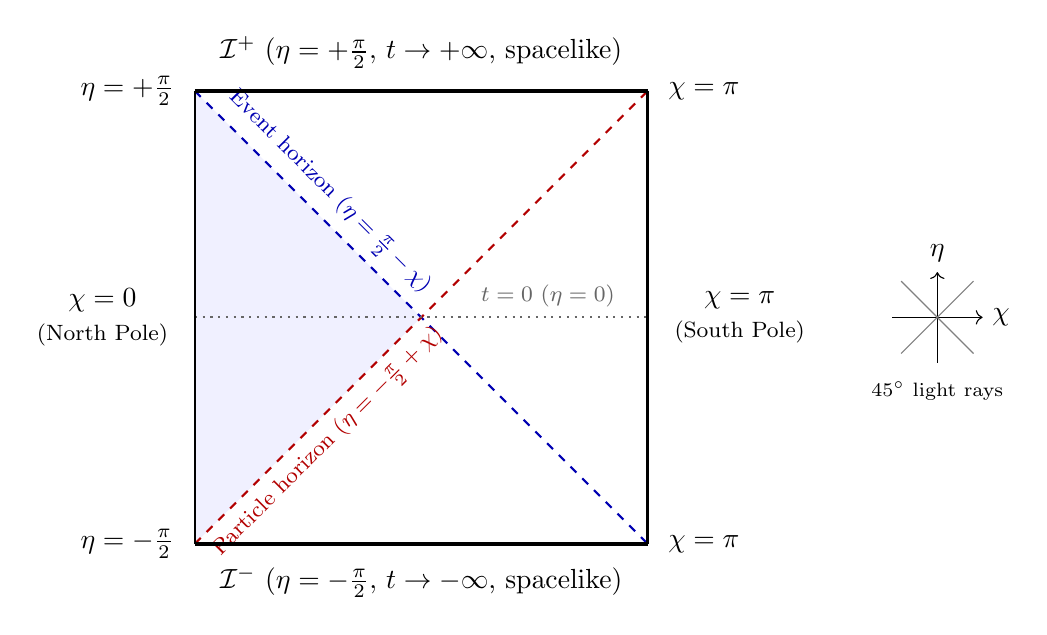
\begin{tikzpicture}[scale=1.15]
  % Shaded causal diamond of observer at chi=0
  \fill[blue!6] (0,-2.5) -- (2.5,0) -- (0,2.5) -- cycle;

  % Horizons (dashed diagonals)
  \draw[dashed, blue!70!black, thick] (0,2.5) -- (5,-2.5) node[pos=0.26, above, sloped, font=\footnotesize] {Event horizon ($\eta = \frac{\pi}{2} - \chi$)};
  \draw[dashed, red!70!black, thick] (0,-2.5) -- (5,2.5) node[pos=0.26, below, sloped, font=\footnotesize] {Particle horizon ($\eta = -\frac{\pi}{2} + \chi$)};

  % Dotted t=0 slice
  \draw[dotted, thick, black!60] (0,0) -- (5,0) node[pos=0.78, above, font=\footnotesize] {$t = 0 \,\, (\eta = 0)$};

  % Main square boundaries
  % Top and Bottom: Spacelike infinity I^+ and I^-
  \draw[ultra thick] (0,2.5) -- (5,2.5) node[midway, above=4pt] {$\mathcal{I}^+$ ($\eta = +\frac{\pi}{2}, \, t \to +\infty$, spacelike)};
  \draw[ultra thick] (0,-2.5) -- (5,-2.5) node[midway, below=4pt] {$\mathcal{I}^-$ ($\eta = -\frac{\pi}{2}, \, t \to -\infty$, spacelike)};

  % Left and Right: Poles of S^3
  \draw[thick] (0,-2.5) -- (0,2.5) node[midway, left=6pt, align=center] {$\chi = 0$\\{\footnotesize (North Pole)}};
  \draw[thick] (5,-2.5) -- (5,2.5) node[midway, right=6pt, align=center] {$\chi = \pi$\\{\footnotesize (South Pole)}};

  % Corner labels
  \node[left=4pt] at (0,2.5) {$\eta = +\frac{\pi}{2}$};
  \node[left=4pt] at (0,-2.5) {$\eta = -\frac{\pi}{2}$};
  \node[right=4pt] at (5,2.5) {$\chi = \pi$};
  \node[right=4pt] at (5,-2.5) {$\chi = \pi$};

  % Lightcone icon placed well to the right of the South Pole label
  \draw[->, thin] (8.2,-0.5) -- (8.2,0.5) node[above] {$\eta$};
  \draw[->, thin] (7.7,0) -- (8.7,0) node[right] {$\chi$};
  \draw[thin, gray] (7.8,-0.4) -- (8.6,0.4);
  \draw[thin, gray] (7.8,0.4) -- (8.6,-0.4);
  \node[below, font=\scriptsize] at (8.2,-0.6) {$45^\circ$ light rays};
\end{tikzpicture}
\end{center}
\end{enumerate}

\vspace{1em}
\hrule

%==============================================================================
% QUESTION 5
%==============================================================================
\ques{6}
\textbf{Problem Statement:} The linearised Einstein equation is
\be
- \frac{1}{2} \partial^\rho\partial_\rho \bh_{\mu\nu} + \partial^\rho \partial_{(\mu} \bh_{\nu)\rho}
- \frac{1}{2} \eta_{\mu\nu} \partial^\rho \partial^\sigma \bh_{\rho\sigma} = 8 \pi G T_{\mu\nu} \,,
\ee
when written in terms of $\bh_{\mu\nu} = h_{\mu\nu} - \frac{1}{2} h \eta_{\mu\nu}$. 

\begin{enumerate}[label=\alph*)]
\item (\emph{1 point}) By making an appropriate gauge choice, explain why the linearised Einstein equation leads to \emph{gravitational waves}.

\medskip
\noindent\textbf{Solution:}

In linearised gravity around flat Minkowski space ($g_{\mu\nu} = \eta_{\mu\nu} + h_{\mu\nu}$ with $|h_{\mu\nu}| \ll 1$), an infinitesimal coordinate (gauge) transformation $x^\mu \to x'^\mu = x^\mu + \xi^\mu(x)$ shifts the metric perturbation by:
\be
h_{\mu\nu} \to h'_{\mu\nu} = h_{\mu\nu} - \partial_\mu \xi_\nu - \partial_\nu \xi_\mu \implies \bh_{\mu\nu} \to \bh'_{\mu\nu} = \bh_{\mu\nu} - \partial_\mu \xi_\nu - \partial_\nu \xi_\mu + \eta_{\mu\nu} \partial_\rho \xi^\rho \,.
\ee
Taking the divergence gives $\partial^\mu \bh'_{\mu\nu} = \partial^\mu \bh_{\mu\nu} - \Box \xi_\nu$ (where $\Box = \partial^\rho\partial_\rho = -\partial_t^2 + \nabla^2$ is the flat-space d'Alembertian wave operator). By choosing $\xi_\nu$ to solve $\Box \xi_\nu = \partial^\mu \bh_{\mu\nu}$, we can always impose the \textbf{Lorenz (or de Donder / harmonic) gauge condition}:
\be
\partial^\rho \bh_{\mu\rho} = 0 \,.
\ee
In this gauge, the second and third terms on the left-hand side of the linearised Einstein equation vanish identically:
\be
\partial^\rho \partial_{(\mu} \bh_{\nu)\rho} = \frac{1}{2}\left(\partial_\mu \partial^\rho \bh_{\nu\rho} + \partial_\nu \partial^\rho \bh_{\mu\rho}\right) = 0 \,, \qquad \partial^\rho \partial^\sigma \bh_{\rho\sigma} = 0 \,.
\ee
The linearised Einstein equation therefore simplifies to the inhomogeneous wave equation:
\be
-\frac{1}{2} \Box \bh_{\mu\nu} = 8\pi G T_{\mu\nu} \quad \Longleftrightarrow \quad \Box \bh_{\mu\nu} = \left(-\frac{\partial^2}{\partial t^2} + \nabla^2\right) \bh_{\mu\nu} = -16\pi G T_{\mu\nu} \,.
\ee
In vacuum ($T_{\mu\nu} = 0$), this reduces to the standard massless relativistic wave equation:
\be
\Box \bh_{\mu\nu} = \left(-\frac{\partial^2}{\partial t^2} + \nabla^2\right) \bh_{\mu\nu} = 0 \quad \left(\text{and equivalently } \Box h_{\mu\nu} = 0\right) \,.
\ee
This admits plane-wave solutions $\bh_{\mu\nu}(x) = \mathrm{Re}\left(\epsilon_{\mu\nu} e^{i k_\rho x^\rho}\right)$ with null wavevector $k_\rho k^\rho = -\omega^2 + |\vec{k}|^2 = 0$, showing that perturbations of the spacetime metric propagate through vacuum as \textbf{gravitational waves} travelling at the speed of light ($c = 1$).

\item (\emph{2 point}) Consider an experiment involving two freely falling test particles, arranged so that one is at spatial position $x^i = (0,0,0)$ and the other at spatial position $x^i=(L_x,0,0)$.
Suppose a gravitational wave travelling along the $z$-axis passes through the laboratory, corresponding to the following metric perturbation:
\be
h_{\mu\nu} = \begin{pmatrix}
0 & 0 & 0 & 0 \\
0 & h_{+}(t-z) & 0 & 0 \\
0 & 0 & - h_{+}(t-z) & 0 \\
0 & 0 & 0 & 0
\end{pmatrix} \,.
\ee
Show that the proper distance between the test particles is given by: 
\be
\Delta s \approx L_x \left( 1 + \frac{1}{2} h_{+}(t) \right) \,.
\ee
If a third test particle is introduced at $x^i=(0,L_y,0)$ show that the proper distance between it and the particle at the origin is
\be
\Delta s \approx L_y \left( 1 - \frac{1}{2} h_{+}(t) \right) \,.
\ee

\medskip
\noindent\textbf{Solution:}

\noindent\textbf{1. Motion of freely falling test particles in TT gauge:}

First, let us verify that a freely falling test particle initially at rest ($u^\mu = \frac{dx^\mu}{d\tau} = (1,0,0,0)$ at $t = 0$) remains at constant spatial coordinates $x^i = \text{const}$ in this coordinate system (which is in Transverse-Traceless, or TT, gauge). The geodesic equation is:
\be
\frac{d u^\mu}{d\tau} + \Gamma_{\alpha\beta}{}^\mu u^\alpha u^\beta = 0 \,.
\ee
For a particle initially at rest ($u^i = 0, u^0 = 1$), the initial coordinate acceleration is determined by $\Gamma_{00}{}^\mu$:
\be
\left.\frac{d u^\mu}{d\tau}\right|_{\text{rest}} = -\Gamma_{00}{}^\mu = -\frac{1}{2} \eta^{\mu\nu} \left( 2 \partial_0 h_{\nu 0} - \partial_\nu h_{00} \right) \,.
\ee
Since $h_{0\nu} = 0$ for all $\nu$ in the given metric perturbation, we have $\Gamma_{00}{}^\mu = 0$ everywhere and at all times! Thus, $\frac{du^i}{d\tau} = 0$, which means the test particles remain at their fixed coordinate positions:
\begin{itemize}
\item Particle 1 remains at $x^i = (0,0,0)$,
\item Particle 2 remains at $x^i = (L_x,0,0)$,
\item Particle 3 remains at $x^i = (0,L_y,0)$.
\end{itemize}

\noindent\textbf{2. Proper distance along the $x$-axis:}

The full spacetime metric is $g_{\mu\nu} = \eta_{\mu\nu} + h_{\mu\nu}$:
\be
ds^2 = -dt^2 + \left(1 + h_{+}(t-z)\right) dx^2 + \left(1 - h_{+}(t-z)\right) dy^2 + dz^2 \,.
\ee
Consider the spatial curve connecting Particle 1 at $(0,0,0)$ and Particle 2 at $(L_x,0,0)$ at constant time $t$ ($dt = 0$) in the $z = 0, y = 0$ plane ($dy = dz = 0$). Along this curve, the line element is:
\be
ds^2 = g_{xx}(t,z=0) \, dx^2 = \left(1 + h_{+}(t)\right) dx^2 \implies ds = \sqrt{1 + h_{+}(t)} \, dx \,.
\ee
Integrating from $x = 0$ to $x = L_x$, and using the binomial expansion $\sqrt{1 + \epsilon} = 1 + \frac{1}{2}\epsilon + \mathcal{O}(\epsilon^2)$ to first order in the small perturbation $|h_{+}(t)| \ll 1$:
\begin{align}
\Delta s &= \int_0^{L_x} \sqrt{1 + h_{+}(t)} \, dx \nonumber\\
&= L_x \sqrt{1 + h_{+}(t)} \nonumber\\
&\approx L_x \left( 1 + \frac{1}{2} h_{+}(t) \right) \,.
\end{align}

\noindent\textbf{3. Proper distance along the $y$-axis:}

Similarly, consider the spatial curve connecting Particle 1 at $(0,0,0)$ and Particle 3 at $(0,L_y,0)$ at constant time $t$ ($dt = 0$) along the $y$-axis ($x = z = 0 \implies dx = dz = 0$). The line element along this segment is:
\be
ds^2 = g_{yy}(t,z=0) \, dy^2 = \left(1 - h_{+}(t)\right) dy^2 \implies ds = \sqrt{1 - h_{+}(t)} \, dy \,.
\ee
Integrating from $y = 0$ to $y = L_y$ and expanding to linear order in $h_{+}(t)$ gives:
\begin{align}
\Delta s &= \int_0^{L_y} \sqrt{1 - h_{+}(t)} \, dy \nonumber\\
&= L_y \sqrt{1 - h_{+}(t)} \nonumber\\
&\approx L_y \left( 1 - \frac{1}{2} h_{+}(t) \right) \,.
\end{align}
Notice the quadrupolar nature of the wave: when the proper distance along the $x$-axis stretches ($h_{+}(t) > 0$), the proper distance along the perpendicular $y$-axis compresses by the same fractional amount, and vice versa.

\item (\emph{3 points}) Consider a binary system consisting of two massive bodies in a circular orbit, which are emitting gravitational waves.
Explain \emph{qualitatively} what happens to the system, and sketch the corresponding gravitational wave signal which would be observed by a detector such as LIGO.
You should mention the following terms: \emph{inspiral}, \emph{merger}, \emph{ringdown}, explain how the interferometer detects a wave such as that described in part b), and connect the features of the signal to the physics of the binary pair. 

\medskip
\noindent\textbf{Solution:}

\noindent\textbf{1. How a laser interferometer (such as LIGO) detects the gravitational wave:}

A detector like LIGO is a large Michelson laser interferometer with two perpendicular arms of equal unperturbed length $L_x = L_y = L$ (for LIGO, $L = 4\text{ km}$) oriented along the $x$ and $y$ axes. A coherent laser beam is split at a central beamsplitter (acting as the test mass at the origin), travels down the two perpendicular arms to suspended, freely-falling mirrors (acting as the test particles at $(L,0,0)$ and $(0,L,0)$), reflects off them, and recombines at the photodetector.

As shown in part b), when a gravitational wave passes through the detector, one arm stretches while the perpendicular arm compresses:
\be
\Delta s_x(t) \approx L \left(1 + \frac{1}{2} h_{+}(t)\right), \qquad \Delta s_y(t) \approx L \left(1 - \frac{1}{2} h_{+}(t)\right) \,.
\ee
This induces an oscillating proper length difference between the two arms:
\be
\Delta L(t) = \Delta s_x(t) - \Delta s_y(t) \approx L \, h_{+}(t) \,.
\ee
Because light always travels at constant speed $c = 1$ along null geodesics ($ds^2 = 0$), the round-trip travel time of light in the $x$-arm increases by $2\Delta s_x / c$ while in the $y$-arm it decreases by $2\Delta s_y / c$. The difference in round-trip light travel times $\Delta T(t) = \frac{2 \Delta L(t)}{c} = \frac{2L}{c} h_{+}(t)$ produces a time-dependent phase shift $\Delta \phi(t) = \frac{4\pi L}{\lambda_{\text{laser}}} h_{+}(t)$ between the two recombined laser beams, which is measured as an oscillating interference intensity pattern at the photodetector.

\medskip
\noindent\textbf{2. Qualitative evolution of the binary system and connection to the signal:}

A binary system of two massive compact objects (such as two black holes or neutron stars) in a circular orbit has a time-varying mass quadrupole moment $I_{ij}(t)$, which sources gravitational waves at twice the orbital frequency ($f_{\text{GW}} = 2 f_{\text{orb}}$). These gravitational waves carry energy and angular momentum away from the binary system to infinity. The evolution proceeds through three distinct stages:

\begin{enumerate}[label=\textbf{\arabic*.}]
\item \textbf{Inspiral:}
\begin{itemize}
\item \emph{Physics of the binary:} As gravitational waves carry energy away ($\frac{dE_{\text{orb}}}{dt} = -P_{\text{GW}} < 0$), the total mechanical energy of the bound circular orbit ($E_{\text{orb}} = -\frac{G m_1 m_2}{2R}$) becomes more negative. Consequently, the orbital separation $R$ decreases. By Kepler's third law ($\Omega_{\text{orb}} = \sqrt{\frac{G(m_1+m_2)}{R^3}}$), as $R$ shrinks, the orbital frequency $\Omega_{\text{orb}}$ and orbital velocities $v \sim \sqrt{GM/R}$ \textbf{increase}. Because the gravitational wave luminosity increases steeply with decreasing separation ($P_{\text{GW}} \propto R^{-5}$), the rate of orbital decay accelerates in a runaway process: the two bodies spiral towards each other faster and faster.
\item \emph{Features of the signal:} In the early inspiral (when $R$ is large), the signal is an almost monochromatic sinusoid with slowly increasing frequency and amplitude. As the orbital separation $R$ shrinks more rapidly, both the \textbf{frequency} ($f_{\text{GW}} = \Omega_{\text{orb}}/\pi \propto R^{-3/2}$) and the \textbf{strain amplitude} ($h \propto \ddot{I} \propto \Omega_{\text{orb}}^2 R^2 \propto R^{-1}$) increase simultaneously, producing the characteristic upward-sweeping \textbf{``chirp''} waveform.
\end{itemize}

\item \textbf{Merger:}
\begin{itemize}
\item \emph{Physics of the binary:} Eventually, the orbital separation shrinks to the scale of the horizons / innermost stable circular orbit (ISCO), where orbital velocities approach a significant fraction of the speed of light ($v \sim c$) and weak-field approximations break down. In this strong-field, highly non-linear regime of general relativity, the two bodies plunge together and coalesce into a single, highly distorted, rapidly rotating remnant object (e.g., a single black hole).
\item \emph{Features of the signal:} The gravitational wave strain $h(t)$ reaches its \textbf{maximum peak amplitude} and a high frequency determined by the total mass of the binary ($f_{\text{merger}} \sim \frac{c^3}{G M_{\text{tot}}}$).
\end{itemize}

\item \textbf{Ringdown:}
\begin{itemize}
\item \emph{Physics of the binary:} Immediately after coalescence, the newly formed remnant black hole is asymmetrical and excited. By the no-hair theorem, it rapidly sheds its multipole deformations by radiating gravitational waves in its characteristic \emph{quasinormal modes} (damped oscillations of the horizon geometry), settling down into a stationary, axisymmetric Kerr black hole.
\item \emph{Features of the signal:} The gravitational wave signal takes the form of an \textbf{exponentially damped sinusoid} (like a struck bell ringing down to silence), with a constant oscillation frequency and damping time determined uniquely by the final mass and spin of the remnant black hole.
\end{itemize}
\end{enumerate}

\medskip
\noindent\textbf{3. Sketch of the Gravitational Wave Signal:}

\begin{center}
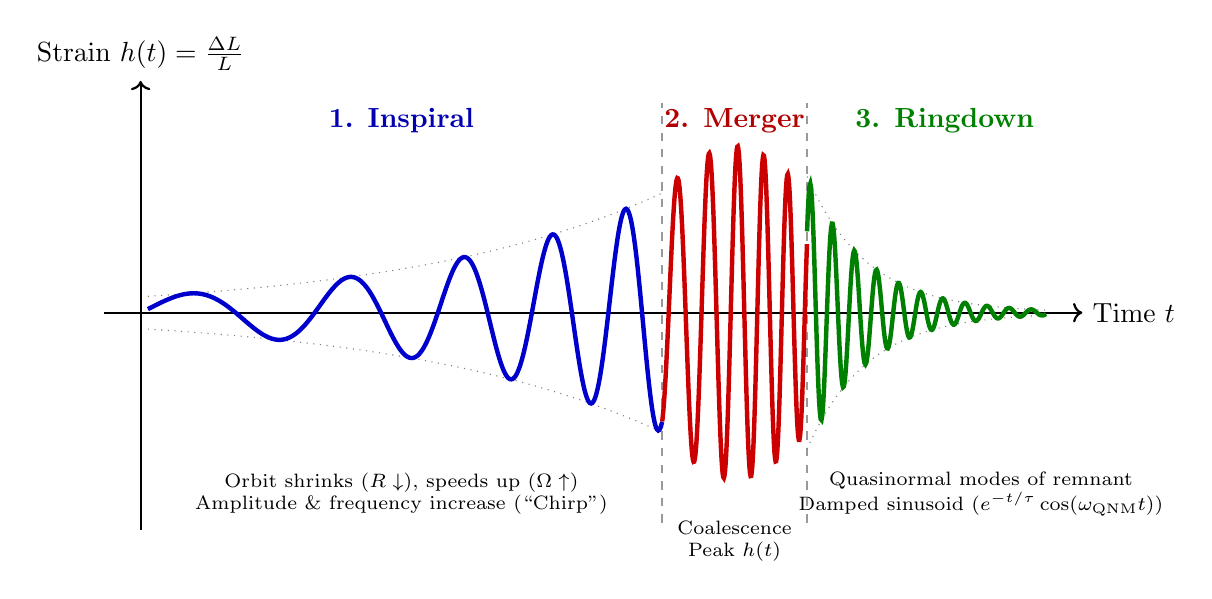
\begin{tikzpicture}[scale=0.92]
  % Axes
  \draw[->, thick] (-0.5, 0) -- (13.0, 0) node[right] {Time $t$};
  \draw[->, thick] (0, -3.0) -- (0, 3.2) node[above] {Strain $h(t) = \frac{\Delta L}{L}$};

  % Region dividers
  \draw[dashed, gray!80, thick] (7.2, -2.9) -- (7.2, 2.9);
  \draw[dashed, gray!80, thick] (9.2, -2.9) -- (9.2, 2.9);

  % Region labels at top
  \node[font=\bfseries, blue!70!black] at (3.6, 2.65) {1. Inspiral};
  \node[font=\bfseries, red!70!black] at (8.2, 2.65) {2. Merger};
  \node[font=\bfseries, green!50!black] at (11.1, 2.65) {3. Ringdown};

  % Envelope (faint) for clarity
  \draw[dotted, gray] plot[domain=0.1:7.2, samples=100] (\x, {0.22 * exp(0.28*\x)});
  \draw[dotted, gray] plot[domain=0.1:7.2, samples=100] (\x, {-0.22 * exp(0.28*\x)});
  \draw[dotted, gray] plot[domain=9.2:12.5, samples=100] (\x, {1.88 * exp(-1.2*(\x-9.2))});
  \draw[dotted, gray] plot[domain=9.2:12.5, samples=100] (\x, {-1.88 * exp(-1.2*(\x-9.2))});

  % Waveform plot:
  % Inspiral: x from 0.1 to 7.2, increasing amplitude and frequency
  % Merger: x from 7.2 to 9.2, peak amplitude and high frequency
  % Ringdown: x from 9.2 to 12.5, exponentially decaying amplitude, high constant frequency
  \draw[ultra thick, blue!80!black] plot[domain=0.1:7.2, samples=400] 
    (\x, {0.22 * exp(0.28*\x) * sin(deg(2.2*\x + 0.12*\x*\x + 0.022*\x*\x*\x))});

  \draw[ultra thick, red!80!black] plot[domain=7.2:9.2, samples=250] 
    (\x, {(1.65 + 0.65*sin(deg((\x-7.2)*1.57))) * sin(deg(2.2*7.2 + 0.12*7.2*7.2 + 0.022*7.2*7.2*7.2 + 12.6*(\x-7.2) + 2.0*(\x-7.2)*(\x-7.2)))});

  \draw[ultra thick, green!50!black] plot[domain=9.2:12.5, samples=300] 
    (\x, {1.88 * exp(-1.2*(\x-9.2)) * sin(deg(2.2*7.2 + 0.12*7.2*7.2 + 0.022*7.2*7.2*7.2 + 12.6*2.0 + 2.0*2.0*2.0 + 20.6*(\x-9.2)))});

  % Annotations below
  \node[align=center, font=\scriptsize] at (3.6, -2.5) {Orbit shrinks ($R \downarrow$), speeds up ($\Omega \uparrow$)\\Amplitude \& frequency increase (``Chirp'')};
  \node[align=center, font=\scriptsize] at (8.2, -3.15) {Coalescence\\Peak $h(t)$};
  \node[align=center, font=\scriptsize] at (11.6, -2.5) {Quasinormal modes of remnant\\Damped sinusoid ($e^{-t/\tau}\cos(\omega_{\text{QNM}} t)$)};
\end{tikzpicture}
\end{center}

\end{enumerate}

\end{document}
